\documentclass[12pt, a4paper]{report}
\usepackage[titletoc]{appendix}
\usepackage{graphicx}
	\graphicspath{{images/}} 
\usepackage{geometry}
	\geometry{a4paper,left=3cm,top=3cm,bottom=3cm,right=3cm}
\usepackage{array}
\usepackage{multirow}
\usepackage{hyperref}
	\hypersetup{colorlinks=true,allcolors=blue}
\usepackage{hypcap}
\usepackage{csquotes}
\usepackage{subfig}

\setlength{\parindent}{1cm}
\setlength{\parskip}{0.1cm}


\begin{document}

\begin{titlepage}
 \begin{center}

\textbf{Progress Report}
\vspace{1cm}

\textbf{\large Software Modelling Learning Gamification}
\vspace{1cm}

Alfa Ryano Yohannis\\
ary506@york.ac.uk
\vspace{1cm}

Supervisor:\\
Dimitris Kolovos\\
Fiona Polack\\
\vspace{1cm}

Department of Computer Science\\
University of York\\
United Kingdom\\
\vspace{1cm}
\today
 
\vfill
 
\end{center}
\end{titlepage}


\begin{abstract}
\addcontentsline{toc}{chapter}{Abstract}
In software engineering, software modelling plays a significant role. Nevertheless, learners often consider software modelling as a comparatively difficult subject since it requires them to have abstraction skills to master it. Meanwhile, gamification has been growing as a trend solution to improving learners' engagement. This study endeavours to harness gameful design to build gamification that supports learners advancing their modelling abilities. Our method to dealing with gameful design combines pedagogical design principles derived from several learning models and the Deterding's Gameful Design framework as an approach to gamification development. This research also employs Model-Driven Engineering best practices and uses the Design Science Research Methodology. This research aims to produce software modelling learning gamification (SMLG), and an SMLG framework to design and generate the SMLG's instances. We plan to perform controlled experiments to evaluate the effectiveness of the SMLG and the SMLG framework.

\end{abstract}

\tableofcontents
\addcontentsline{toc}{chapter}{Contents}

\chapter{Introduction}
\label{Introduction}


The nature/main problems of modelling.

Opportunity to use games.

Motivations, needs, desired qualities.

Existing approaches of using games to address the problems.

The lack of existing problems and rooms for improvements.

Motivations, needs, desired qualities.

Proposed solutions.

-------------------------
Methodology

Identify Problem and Motivation
- Part of this are in the introduction 
- Research Question

Define Objective and Solution
- Research Objectives
- Research Solution
- Research outcomes
- Contribution to environment
- Contribution to knowledge

Design and Development
- Requirements
- Grounding
- Ethical Consideration
- Design
- Development

Demonstration and Evaluation

Communication
- Publication

-------------------------------------------
Research Plan
- Complete Basic Functionality
- Improve usability
- Design Experiments for Evaluation
- Publication


Software modelling is commonly perceived as a difficult subject since it requires a mastery of abstraction \cite{Borstler2012}. However, this subject has a fundamental and crucial role in software engineering education and practice. Successful application of software modelling requires skills in abstract modelling \cite{whittle2013industrial}. The modelling itself is the process of thinking abstractly about systems \cite{bezivin2009teaching}. Thus, teaching modelling also means teaching abstraction \cite{engels2005teaching}. Therefore, it is crucial to make students understand the value of abstraction \cite{bezivin2009teaching}. Weak software modelling skills will likely cause software engineering students to face further challenges with their degrees, as most of the software engineering related subjects involve of inherent abstraction problems \cite{Kramer2007}. In the context of computer science and software engineering education, Kramer \cite{Kramer2007} and Hazzan \cite{hazzan2008reflections} argued that abstraction is the central theme or key skill for computing.

\begin{displayquote}
``I believe that abstraction is a key skill for computing. It is essential during requirements engineering to elicit the critical aspects of the environment \dots At design time \dots Even at the implementation stage \dots --- Kramer \cite{Kramer2007}.
\end{displayquote}

\begin{displayquote}
`` \dots software is an intangible object, and hence, requires highly developed cognitive skills for coping with different levels of abstraction." --- Hazzan \cite{hazzan2008reflections}.
\end{displayquote}

The problem of learning appropriate abstraction skills for software modelling is similar to problems in mathematics, where most of the concepts can only be accessed through symbolical representations \cite{Duval2006}. Abstraction also requires students to grasp skills in information hiding, generalisation, approximation or reformulation and separating relevant from irrelevant aspects \cite{Saitta2013}. To overcome these challenges, we need to put effort into software modelling learning design, developing a concrete and motivating presentation which can engage students and facilitate deep learning.

In recent years, the use of games and game elements for purposes other than leisure has drawn significant attention. Gamification \cite{deterding2011game} and Serious Games \cite{Michael2005} (we use `gamification' to refer to both concepts) have been proposed as solutions to motivational problems that emerge when users are required to engage in activities that they perceive as boring, irrelevant, or difficult. Figure \ref{gamification-trend} shows the growth of ``Gamification" on Google Trends\footnote{\url{https://www.google.com/trends/explore?date=all&q=\%22gamification\%22}} since February 2010. 

\begin{figure}[ht]
\centering
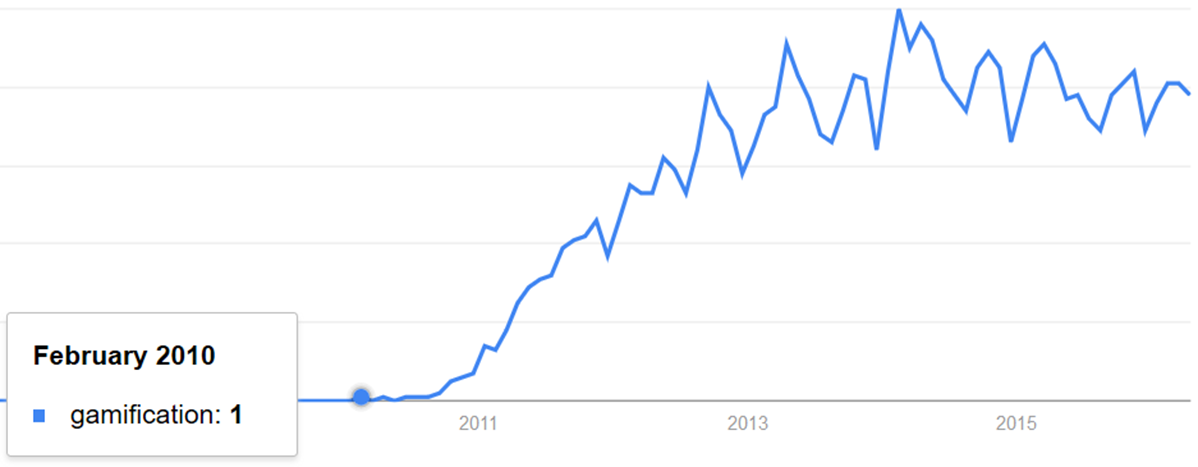
\includegraphics[width=12cm]{gamification-trend}
\caption{``Gamification" on Google Trends per 12 April 2016.}
\label{gamification-trend}
\end{figure}

Real-world examples that show the success of the gamification are Duolingo\footnote{\url{https://www.duolingo.com/
}} and Re-mission\footnote{\url{http://www.re-mission.net/}}. Duolingo is a gamified system of language learning. It embeds game elements, such as points, levels, and lives, to make language learning more fun. Re-mission is a third-person shooting game dedicated to young cancer patients and designed to teach and learn how to deal with cancer. The patients are invited to take part in an entertaining gameplay that will affect their specific behavioural and psychological outcomes producing effective cancer therapy.
 
Through a systematic review, Connolly et al. \cite{connolly2012systematic} studied the impact of computer games and serious games on engagement and learning in diverse fields. They reported the majority of the studies presented empirical evidence about the positive impact of computer games and serious games. Using the same type of method, Hamari et al. \cite{hamari2014does} found that according to the majority of the reviewed papers, gamification does generate benefits and positive effects. Specifically in the field of software engineering, Pedreira et al. \cite{Pedreira2015} also performed a systematic review on the application of gamification in software engineering. Most existing studies focus on software development, project management, requirements, and other support areas, but none of them focuses on software modelling. They also found fewer studies reporting empirical evidence to support gamification research. They argued that existing studies in the field are quite new, thus more research effort is needed to investigate the impact of gami�cation in software engineering. 

Reports of the positive impact of gamification in various fields encourage us to apply it in software modelling learning, an area which has received little attention for the application of gamification so far. This situation broadens our opportunity not only to produce a novel approach to teaching software modelling but also to improve gamification processes through the application of Model-Driven Engineering approaches. This research proposes a main research question, ``Can gamification improve software modelling learning?". The word `improve' implies that learning with gamification enhances learners' engagement and learning performance. The engagement of learners with the support of gamification is more durable, frequent, and active compared to learners that only use didactic approach. Also, the former perform better in knowledge and skill acquisition and application compared to the latter.   

In the beginning, we plan to address software modelling in Model-Driven Engineering as a whole---comprising modelling, metamodelling, and model transformation. However, after consideration regarding scope and time, we adjust our scoping just to focus on graphical software modelling, which is a common way to express models in modelling and metamodelling. We excluded model transformation since its approaches are commonly expressed in a textual way. We include metamodelling since a metamodel itself is a model of models and usually is expressed in the form of class diagram-like graphics. We plan to perform literature study and develop a prototype in the first year and address modelling and metamodelling in the second year and third year respectively. 
    
Instead of developing the software modelling games manually, we plan to follow a model-based approach. We will develop a design framework for the games, which will systematically and semi-automatically drive gamification design to produce software modelling learning gamification (SMLG). We call the framework the SMLG framework. Essentially, our study lies in the intersection between software modelling, learning, and games as depicted in Figure \ref{smlg}. Therefore, pedagogical aspect cannot be neglected. We will apply several learning models from pedagogy to drive the design of our learning game. We also target the SMLG is suitable for higher-level undergraduate and postgraduate students with some of experience of software engineering. 

The remainder of this report is organised as follows. We provide a detailed literature review in Section 2 and propose the research proposal as well as the research methodology in Section 3. Finally, in Section 4, we end this qualifying dissertation with a discussion on our preliminary results. 

\begin{figure}[ht]
\centering
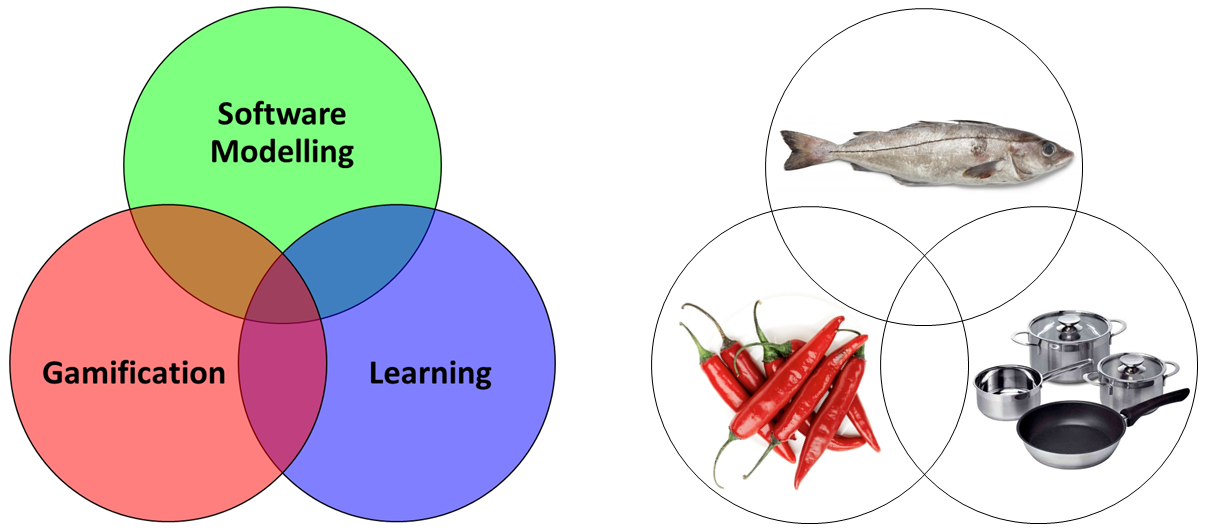
\includegraphics[width=\textwidth]{smlg}
\caption{How to 'Cook' a Gameful Software Modelling Learning?}
\label{smlg}
\end{figure}

Grounded on the literature review in Chapter \ref{Field Survey and Review}, in this section, we present our research questions as well as our research aim and objectives to answer the questions. We also present the possible research outputs that will be produced by our research and the research methodology that we are going to apply to address the research questions.   

\section{Research Questions}
The main research question proposed by this research is ``Can gamification
improve software modelling learning?". The word `improve' implies that learning
with gamification enhances learners' engagement and learning performance.
Learners with the support of gamification engage more durable, frequent, and
active compared to learners that only use didactic approach. Also, the former
ones perform better in knowledge and skill acquisition and application compared
to the latter ones. To answer the main research question, following sub research
questions need to be investigated:
\begin{enumerate}
\item Which parts of software modelling teaching and learning could benefit from gamification?
\item What teaching and learning best practices of software modelling that are significant to be accommodated in SMLG?
\item What pedagogical learning models and in what roles that can improve the engagement and effectiveness of SMLG?
\item What kind of gamification design that can support software modelling learning best? 
\item What kind of orchestrating framework is needed to design the interaction between software modelling and game elements to achieve effective SMLG?
\item To what extent does SMLG improve learners' motivation, engagement, and performance?
\item To what extent do software modelling tutors benefit from a SMLG framework?
\end{enumerate}

\section{Objectives}
\label{Objectives}
The main aim of this research is to assess to what extent gamification can improve software modelling learning. Therefore, we will investigate and develop an SMLG framework that systematically and semi-automatically drives gamification design and generation to produce SMLG. More precisely, this research aims to meet the following research objectives that are derived from the main research aim:

\begin{enumerate}
\item Perform a literature review to identify research problems, questions, and objectives. 
\item Develop a framework that is intended to design and generate SMLG based on the literature review and survey. The framework will be iteratively updated according to the results obtained from experiments. 
\item Design and generate instances of SMLG. The instances will be tested to respondents for evaluation and to obtain feedback for iterative improvement. 
\item Perform controlled experiments to measure the significance of the SMLG in improving learning performance compared to traditional method, didactic learning without the support of the gamification.
\item Perform controlled experiments to measure the productivity and maintainability of a software modelling learning design framework in supporting tutors design and develop SMLG. 
\end{enumerate}

\section{Research Outputs}
The potential research outputs of this research are:
\begin{enumerate}
\item Software/applications of SMLG. The applications/instances of SMLG that are designed and generated using a SMLG framework. 
\item A framework for designing and generating applications of SMLG.
\item Controlled experiments: a learning outcome comparison between gamified version and the traditional one of software modelling learning.
\item A model that explains how SMLG works. The model can be achieved through Learning and Game Analytics and Structural Equation Modelling studies.
\item Case studies: reports of applications of theories, models, and methods used in this research.
\end{enumerate}



Your introduction to your research and research area can be quite short, but needs to make sense to someone who did not read (or does not remember) your QD.  

You should reiterate the motivation for your research (e.g. the gap that it is intended to fill). You should also state succinctly any changes to the scope of your research since the QD milestone: if you have not changed scope or direction, say so.

Be clear what hypothesis or research questions you are addressing and why.

\chapter{Progress Review}
\label{Progres Review}

In this section, we present our preliminary results. First, we present the
result of our preliminary survey regarding the needs, motivation, and challenges
of software modelling learning from the perspective of Model-Driven Engineering
module's students. Next, we summarise our literature review regarding best
practices in software modelling teaching into lists of design requirements.
After that, we elaborate the potential contribution of the discussed learning
models to the design of the SMLG. In the end, we present the preliminary design
of the SMLG as well as the SMLG framework.

\section{Research Methodology}
In this section, we discuss briefly the research methodology that we apply to
address research questions presented previously. Since the main outputs are
design artefacts---the applications of SMLG and the SMLG framework to generate
them, Design Science Research Methodology \cite{peffers2007design} is selected
as the research method as it provides a comprehensive conceptual framework and
activity guidelines for understanding, developing, executing, and evaluating the
design artefact. We also discuss briefly our evaluation plan to evaluate our
research findings. In the end of this section, we present our Research Data
Management approach as part of good research practices.

\subsection{Design Science Research Methodology}
We will employ Design Science Research Methodology \cite{peffers2007design} as
the methodology to carry out the research. DSRM is selected since it provides a
comprehensive conceptual framework that consists of activity guidelines for
understanding, developing, executing, and evaluating design artefacts (Figure
\ref{dsrm}). Another reason is that it positions itself at the top level of
abstraction without going into much detail of how to perform each activity, we
can freely choose other more concrete research methods to carry out the
activities. For examples, we can conduct literature reviews, surveys, or expert
interviews to determine research problems, motivations, solutions, and
objectives as well as controlled experiments to measure and evaluate the
effectiveness of the artefacts.

\begin{figure}[ht] \centering 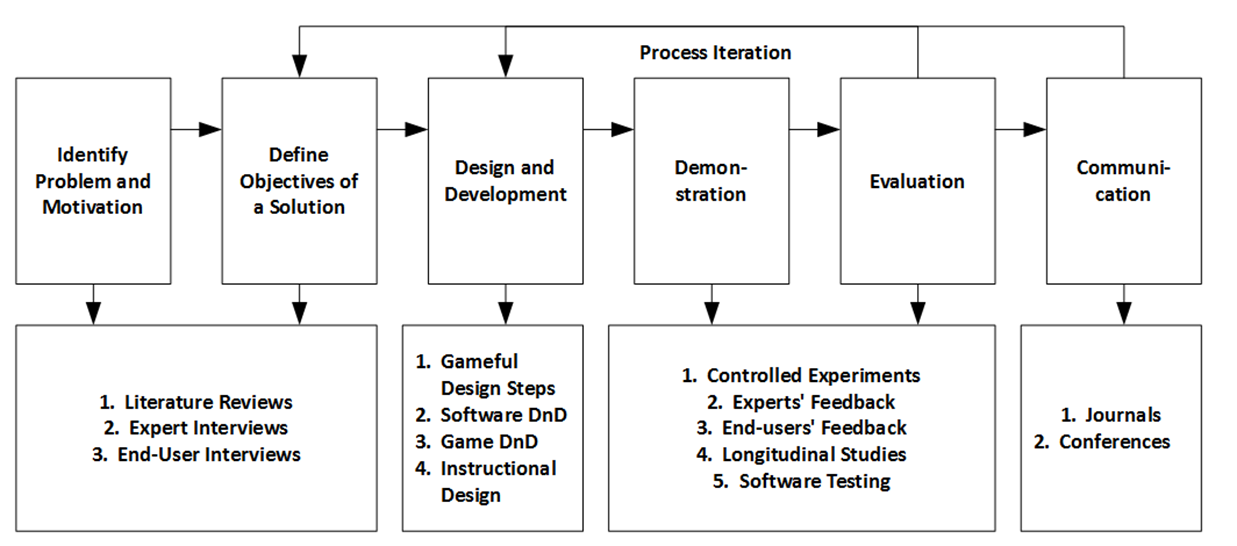
\includegraphics[width=\textwidth]{dsrm}
\caption{Design Science Research Methodology. Adapted from Peffer et al. \cite{peffers2007design}.}
\label{dsrm}
\end{figure}

\textbf{Identify Problem and Motivation}. This research will use literature review, suggestions from experts, and surveys to identify research problems and motivations as the background to determine the solution and its objectives. The experts are academicians or practitioners that have significant experience in Model-Driven Engineering and respondents are the students of Model-Driven Engineering-like modules (Software Analysis and Design, Model-Driven Software Development, etc.). In this way, (1) we can identify parts of software modelling teaching and learning that could benefit from gamification, (2) we can also determine software modelling teaching and learning best practices that are significant to be accommodated in SMLG, (3) we are facilitated to decide which pedagogical learning models that can improve the engagement and effectiveness of SMLG, as well as (4) to determine what kind of gamification design that can support software modelling learning best. Performing problem and motivation identification addresses research questions one to four.  

\textbf{Define Objectives of a Solution}. Based on the identified problems and motivations, we define our solution that is embedding gamification in the process of software modelling learning, which is expressed by the use of gamification applications specifically designed for software modelling learning. Research objectives have been defined in the previous section (section \ref{Objectives}).

\textbf{Design and Development}. This research will employ Gameful Design
Framework \cite{deterding2015lens} to design and develop the SMLG and agile
software development \cite{stober2010overview} to design and develop the
software/applications. The design and development activities are part of the
iterative cycles and the products of the activities will be refined as required
based the results generated from the evaluation activity. For the framework that
generates the SMLG, we build one application of SMLG that addresses one
graphical modelling language. From there, we make an abstraction of reusable
components of the application and implement Model-Driven Engineering approaches,
such as modelling, metamodelling, and code generation, to generate different
applications specific for other graphical modelling languages.

\textbf{Demonstration and Evaluation}. The resulting applications and the
framework to generate them will be demonstrated and evaluated by applying it to
several courses of software modelling. Moreover, the evaluation results will be
used as feedback to improve the quality of the applications and the framework
and as a ground to judge the research findings. Demonstration and evaluation
activities are parts of the iterative cycles and will be performed again as
required.

\textbf{Communication}. Significant findings will be published in an academic conferences or journals for dissemination and evaluation by the related research communities.

\subsection{Evaluation}
We plan to evaluate (1) the effectiveness of the SMLG discussed above and (2) the productivity and maintainability benefits of the SMLG framework. For the effectiveness evaluation, controlled experiments will be used. The participants, software modelling students, will be divided into two groups, a control group and an experimental group. The control group will learn software modelling using traditional methods while the experimental group will learn with support from the SMLG. Then, their performance of the two groups will be measured by their ability to solve a set of related modelling problems. 

For the evaluation of the SMLG framework, the participants will be software modelling tutors; they will be divided into two groups, one that will develop SMLG \emph{with} the SMLG framework and one \emph{without} the SMLG framework (i.e. using existing web technologies). They will be asked to elaborate their SMLG into their teaching instructions and use them in their teaching. The comparison will be on their productivity and the maintainability of their SMLG. To evaluate the generality of the results of both evaluation processes, conducting experiments in different years and countries is also considered.

Additionally, surveying with questionnaires or interviews might be conducted to investigate the underlying variables or processes. Structural equation modelling \cite{hair2016primer} is also an option if measuring the effects of the identified underlying variables is required. An alternative method for understanding of the underlying variables and processes is through investigating the SMLG's event logs using data mining or machine learning techniques.

\subsection{Research Data Management}
During the evaluation phase of this project, we plan to collect data from our respondents---part of research that is sensitive to privacy issues. Thus, as part of good research practices at the University of York\footnotemark \footnotetext{\url{https://www.york.ac.uk/library/info-for/researchers/data/}}, Research Data Management (RDM) is obligatory to ensure our research protects the privacy of our respondents, conforms to the law, and respects research ethics, as well as to demonstrate research excellence and integrity. Therefore, we plan to design a Data Management Plan (DMP) that refers to the Digital Curation Centre's outlines, which means the plan should address the following six main points: (1) Data Types, Formats, Standards, and Capture Methods. (2) Ethics and Intellectual Properties. (3) Access, Data Sharing, and Reuse. (4) Short-Term Storage and Data Management. (5) Deposit and Long-Term Preservation. (6) Outsourcing \cite{jones2011develop}. To support our work, we will use the DMP template\footnotemark[\value{footnote}] provided by the University of York for postgraduate research projects.



\section{Preliminary Survey}
\label{Preliminary Survey}
In this research, we have conducted our preliminary survey to identify learners' needs, motivations, and challenges according to the Research phase of the Deterding's Gameful Design Framework. The preliminary survey is not intended to measure significance, but it is more to qualitative investigation to reveal needs, motivations, and challenges in learning software modelling from learners' perspective.    The preliminary survey is also in line with the Design Science Research Methodology, in order to identify the problem and motivation so that we can define objectives of a solution accurately in the second activity. 

We have distributed online questionnaires to students of Model Driven
Engineering (MODE) 2015/2016 module. The students were in their Software
Engineering master programme at the University of York. From 21 students, only 4
completed the questionnaires. Their responses can be found in Appendix
\autoref{chap:Preliminary Survey Data}.  Since the number of respondents are
small for generalisation, we plan to apply the same survey to next term MODE
students.

\textbf{Results}. To identify the learners' needs, we asked our respondents two questions. Question 1 aims to identify students' expectations before starting the module, while question 2 aimed at identifying what the students found important after taking the module. Based on the responses, the reasons why the students took MODE module because they want to increase their knowledge on MDE, possess new advanced skills or abilities and improve their literation of MDE tools. After completing the module, the students valued that the most important lessons were getting new knowledge---domain modelling, metamodel, abstract syntax, abstract thinking, model validation, and the application of models---and skills---generating code, creating DSL, and improving their tool skills. 

We also asked the students three questions (Q3-Q5) to identify their motivation
in taking MODE module and Learning Model Driven Engineering. Question 3 asked
about the reasons behind their decision taking MODE module. Two students stated
that they took the module because it is compulsory, but the rest of the students
said that they took the module because MDE is an advanced topic and they wanted
to see its applicability in the industry and whether it will improve their
ability---knowledge and skills.

Question 4 asked the students about what would motivate them more to learn Model
Driven Engineering (MDE). The students responded that they would be more
motivated if they could perceive the advantages of MDE: efficiency and
effectiveness it could offer, the benefits of its application in the
organisation or real world examples, and its genericity---MDE application in
languages other than Java or models other than UML/EMF.

We then asked question 5 which asked the students the most basic, underlying motives that make them commit to learning MDE. Substantially, they answered that their main motivation is to gain new ability---knowledge and skills, such as the ability to make an abstraction, advanced skills that are applicable in industry, and knowledge of real-life examples and applications of different models taught in MDE. Nevertheless, passing MODE module, a pragmatical motive, still part of the whole motivation. 

In question 6 and 7, we asked the students about the interesting challenges that they faced during MODE module. They mentioned abstract thinking and model management activities such as defining metamodels, validating model, and how to best model a system---satisfying the model's metamodel and validation so the model could be easily queried and transformed). To overcome challenges, what they did are performing trial-and-error method or experimenting the problems, try many other examples, and completing all the practicals. We summarised all of these efforts as activities to build 'experience'.

We also asked them question 8 and 9 about the non-interesting challenges, extraneous challenges that are not relevant to the core activities of modelling. They mentioned following activities: dealing with very specific technical concepts/words that only belong to specific products, focusing too much on how to use tools in other words using very tedious tools or less information on how to use the tools, and judging the quality of a model since there was no explanation of how good of bad the model was. To deal with the uninteresting challenges, they just ignored them, seeking information and solutions from the internet, lecturers, assistants, and discussion groups, and redid building the solutions from the beginning when they had certain problems using the tools.

\textbf{Discussion}. There are few findings from the preliminary interview regarding students' needs, motivations, and challenges, that can be implemented into the design of a SMLG. \textit{First}, the need of the students to learn MDE is to gain new advanced abilities---knowledge and skills---that are applicable in industry, which, if broken drown, they comprise of model management activities (abstract thinking, modelling, metamodelling, model transformation, validation, and application) and tool literacy. 

\textit{Second}, the motivations of the students to learn MDE are, regardless their view on MODE module as a compulsory module in their programme, they were aware that their motivation should be on satisfying their need in gaining advanced knowledge and skills in MDE as mentioned before, and they would be more motivated if they could perceive the advantages and applicability of MDE, thus showing students the benefits and applications of MDE are crucial in increasing their motivation.

\textit{Third}, they mentioned model management activities (abstract thinking, model validation, metamodelling, etc.) as the interesting challenges. To overcome the challenges, they did trial-and-error method to gain more experience in overcoming the challenges. These findings are in line with experiential learning which states learning is best achieved through experiencing \cite{kolb2014experiential}. The main concern of gameful design is to reduce the cost of performing such activities so that learners could focus on the core activities without distraction. It could be done by dividing the activities into smaller activity chunks and removing the extraneous, unrelated activities \cite{deterding2015lens}. 

The extraneous, unrelated activities were identified by asking question 8 and 9, which aimed at determining the uninteresting challenges. Most of the complaints were on the tools which were tedious to use. They also argued that there is no need to learn the detailed technical concepts or terms that were only unique to certain products. To overcome the uninteresting challenges, the students preferred to seek information and solutions from on internet, lectures, and discussion groups. Thus, it is paramount to provide comprehensive documentation and support of the tools used in a learning activity \cite{liebel2015ready}. 

\begin{table}[ht]
\caption{Requirements derived from the preliminary survey (section \ref{Preliminary Survey}).}
\label{table:preliminary-survey}
\begin{center}
\begin{tabular}{ p{2cm}p{1cm}p{10cm} } 
\hline
Category & Code & Requirements from Preliminary Survey \\
\hline
\multirow{1}{2cm}{Needs} 
& RS01 & Teach them knowledge and skills that are applicable in industry: model management (abstract thinking, modelling, metamodelling, model transformation, validation, and application) and tool literacy. \\ 
\hline
\multirow{1}{2cm}{Motivations}
& RS02 & Promote gaining advance knowledge and skills in MDE. \\ 
& RS03 & Promote the benefits and applications of MDE. \\ 
\hline
\multirow{1}{2cm}{Interesting Challenges}
& RS04 & Challenge with model management activities (abstract thinking, model validation, metamodelling, etc.). \\ 
& RS05 & Scaffold learning process to support learners gaining their experience (for an example, dividing the activities into smaller activity chunks). \\ 
\hline
\multirow{1}{2cm}{Un-interesting Challenges}
& RS06 & Increase the usability of the tool being used. \\ 
& RS07 & No need to learn the detailed technical terms specific to certain products. \\ 
& RS08 & Provide documentation and support for the tools being used. \\ 
\hline
\end{tabular}
\end{center}
\end{table}

\section{Design Requirements}
\label{Design Requirements}
Throughout the literature review, we have gathered requirements, which are the
key points pointed out by MDE experts how we should teach MDE. Table
\ref{table:requirements} is a list of requirements summarised from the
literature review in section \ref{Software Modelling Teaching}. These
requirements have two roles. First, they provide guidance to our design process
and, second, they will also act as units of evaluation to confirm the SMLG meets
the current best teaching practices.
 
We also derive other requirements from our preliminary survey in section \ref{Preliminary Survey}. 
These requirements (Table \ref{table:preliminary-survey}) have the same role as other requirements 
derived from the literature review, except that these requirements address the needs, motivations, 
and challenges in designing the gameful aspect of SMLG. From our requirement identification, we found out that the items in the Contents category (Table \ref{table:requirements}) agrees with the item in the Needs category (Table \ref{table:preliminary-survey}). The finding suggests an agreement about the learning contents that should be delivered to students in learning MDE.

\begin{table}[ht]\caption{Requirements derived from the literature review (section \ref{Software Modelling Teaching}).}
\label{table:requirements}
\begin{center}
\begin{tabular}{ p{2cm}p{1cm}p{10cm} } 
\hline
Category & Code & Requirements from Literature Review \\
\hline
\multirow{1}{2cm}{Contents} 
& RL01 & Teach MDE Definition \\ 
& RL02 & Teach semantics, syntaxes, notations \\ 
& RL03 & Teach Modelling, metamodelling, model validation, model transformation\\
& RL04 & Teach the applications of MDE \\
& RL05 & Teach modelling in various domains/contexts \\

\hline
\multirow{1}{2cm}{Priciples and Practices} 
& RL06 & Modelling is abstract thinking \\ 
& RL07 & Object-orientation prerequisite \\
& RL08 & Measure student's model's quality \\
& RL09 & Problem solving first, detail specifications and tools get in the way \\
& RL10 & Provide support to solutions, not answers \\ 
& RL11 & Teach broadly, throughout, not deeply \\
& RL12 & Teach with different modelling languages \\ 
& RL13 & Make it fun \\ 
& RL14 & Teach from ground, real-world objects, up to abstraction \\ 

\hline
\multirow{1}{2cm}{Tool Design}
& RL15 & Support and documentation \\
& RL16 & Build knowledge incrementally \\
& RL17 & Flexibility to explore learning \\
& RL18 & Positive reinforcement \\
& RL19 & Convince of the value of the topic being learned \\ 
& RL20 & High usability \\ 
\hline
\end{tabular}
\end{center}
\end{table}

\section{Elaborating Design and Learning Models}
\label{Elaborating Design and Learning Models}
In section \ref{Pedagogy}, we proposed several existing learning models that we will apply in the design process of our SMLG. In this section, we will explain the relationships between the learning models, their contributions, and how they will be applied to the design of the SMLG are depicted in in Figure \ref{learning-models} and Figure \ref{learning-models2}.

We decided to implement challenge as the fundamental game element that exists in the design of our game since it is one of the key features that exist in every game. The challenge is a crucial game element since it stimulates and provokes a player to engage with SMLG. We translate challenge into series of levels in our design and of course higher levels come with higher difficulty. To realise this, we borrow the learning activities---remember, understand, apply, analyse, evaluate, create---from Bloom's taxonomy, since every activity has different cognitive loads according to their order with 'create' has the highest cognitive load. We assume that activity with higher cognitive load is also harder to complete. Therefore, we can make different combinations between the activities that will gradually increase in difficulty (cognitive load) along the increase of the levels (Figure \ref{learning-models}). Bloom's taxonomy also act as an inventory of activities that provide us many options of activities that could give variability in our design. 

\begin{figure}[ht]
\centering
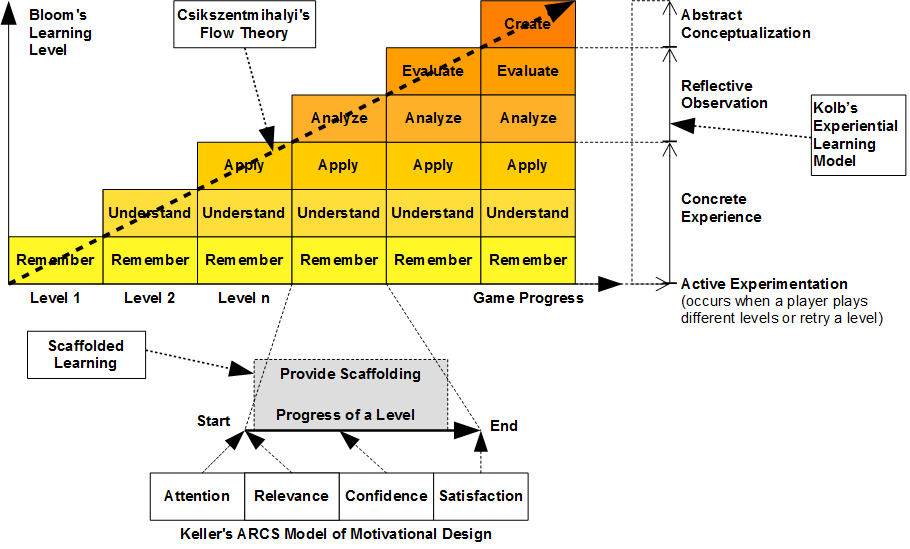
\includegraphics[width=\textwidth]{learning-models}
\caption{Elaborating learning models' contribution to the design of the gamified modeling learning}.
\label{learning-models}
\end{figure}

\begin{figure}[ht]
\centering
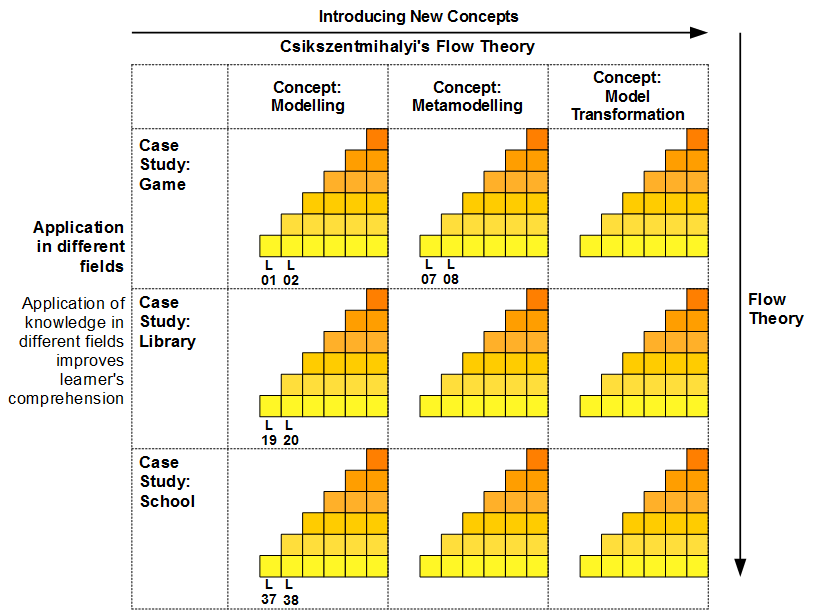
\includegraphics[width=\textwidth]{learning-models2}
\caption{Elaborating learning models' contribution to the design of the gamified modeling learning}.
\label{learning-models2}
\end{figure}

While learners are progressing in the SMLG, they are developing their competence. Thus, difficulty has to be kept balanced with their competence, otherwise they will get bored. It is the situation where the theory of Flow can be applied (Figure \ref{learning-models}). To control degree of difficulty, there are three ways we identified so far related to pedagogical approach: a combination of Bloom's activities, the introduction of new concepts, and application in different domains. The order of the levels of each of the three ways has to be arranged properly following the theory of Flow. Concepts that are easier are given earlier than the harder ones, and the difficulty is increased gradually as learners progress. Likewise, Application in the domains that are more familiar with learners should be given first and gradually shifted to the domains that are most unfamiliar (Figure \ref{learning-models}. Combining these three dimensions---types of activities, concepts, and domains---could give us a variety of levels with different degrees of difficulties.

Motivation is an important aspect in the success of learning, and we use Keller's ARCS motivational model to address this aspect \cite{keller2010motivational}. The model provides us in each its components---attention, relevance, confidence, satisfaction---a set of predefined techniques to maintain learners' motivation. In a course of a level of SMLG, there are a start, an end, and learning activities in between (Figure \ref{learning-models}). We could apply the ARCS' techniques to maintain learners' motivation along the course of completing a level. As an example, we could use animation to gain learners' attention, explaining the application of the concept being taught in the currently playing level to give relevance, showing their progress in completing a level to maintain their confidence, and giving them a reward after finishing a level for reward.
 
We apply scaffolding \cite{vygotsky1978mind, wood1976role} to support learners coping challenges (Figure \ref{learning-models}). Throughout finishing a level, scaffolding could be provided in several ways: reducing extensive modelling activities into smaller activity constituents, removing irrelevant activities, providing an almost complete model so they can work on the most relevant activities rather than build the model from scratch, providing help and documentation, and giving some clues of the solutions when they get stuck. This support will be reduced as players progress to maintain the balance between their increasing competence and difficulty.

We also consider applying Kolb's experiential learning model, which is a model that agrees knowledge is constructed through experience and based its model on constructivism \cite{kolb2014experiential}. We select Kolb's model since we perceive that playing a level in SMLG is similar to the learning cycle Kolb proposed; a cycle consists of 4 steps: concrete experience (CE), reflective observation (RO), abstract conceptualisation (AC), and active experimentation (AE). 

We could apply this cycle to frame learners' activities in gaining new knowledge through solving a problem given in a level. For example, the first time players play a new level, at that moment they encounters a concrete experience (CE). Immediately, they attempt to identify and characterise the problem given in that level and recall any knowledge that is relevant to solve the problem (RO). Next, they construct a solution for the problem that they face (AC). After constructing the solution, they apply the solution to the problem (AE), experience the result (CE), and then evaluate whether the solution solves the problem of the level or not (RO). Any gap that appears will update their knowledge. They use their newly updated knowledge to produce a new solution (AC) that could be applied to the same problem at the same level or different problem in other levels (AE). In case that the player already `game Over' and they cannot apply their new solution, AE occurs when they replay the same level or play a similar level.

\begin{table}[ht]
\caption{Requirements derived from learning models (section \ref{Elaborating Design and Learning Models}).}
\label{design-learning-models}
\begin{center}
\begin{tabular}{ p{2cm}p{1cm}p{10cm} } 
\hline
Category & Code & Requirements from Learning Models \\
\hline
\multirow{1}{2cm}{Learning Models} 
& RM01 & Design satisfies Bloom's taxonomy. \\
& RM02 & Design suffices Kolb's experiential learning model. \\ 
& RM03 & Design meets Keller's ARCS motivational model. \\
& RM04 & Design fulfils scaffolded learning. \\
& RM05 & Design complies with the theory of Flow. \\ 
\hline
\end{tabular}
\end{center}
\end{table}

Learning activities in Bloom's taxonomy also correspond to the steps in Kolb's learning cycle \cite{murphy2007prior} and both have been applied together to design instructions in different fields \cite{terry1993kolb, howard1996felder, schatzberg2002applying}. Therefore, we argued that both could be implemented simultaneously; Bloom's taxonomy provides learning activities while Kolb's model addresses learning cycles in the design of our game. To simplify our work, we summarise the elaboration of design and learning models into a list of requirements (Table \ref{design-learning-models}) that will be used in the design and evaluation activities.

\section{Gamification Design}
\label{Gamification Design}
In this research, we plan to assess whether gamification is beneficial for learners of graphical software modelling languages. We choose graphical modelling languages since they are the common languages used in modelling, whether in academia or industry, and extensively used in Model-Driven Engineering. Standard graphical modelling languages like UML\footnote{\url{http://www.uml.org/}} and BPMN\footnote{\url{http://www.bpmn.org/}}, often used in Model-Driven Engineering, are some of the use-cases.        

Modelling can be expressed in different modelling languages. To minimise bias and ensure the generality of our SMLG, we plan to experiment and support several graphical modelling languages (e.g. UML, BPMN, state-charts). For each modelling language, we envision the development of dedicated SMLG that will be derived from the Gameful Design Framework \cite{deterding2015lens}. The SMLG will mimic a graphical modelling tool, and at each level, it will require the learner to graphically construct or adapt a model to meet a set of constraints and requirements.

The SMLG will have levels of gradually increasing difficulty as well as variety in its challenges, to expose learners to different kinds of domains, models, and diagrams. Tutorials are planned to be embedded into the SMLG to help learners familiarise themselves with the control system and the flow of the SMLG. 

The SMLG will incorporate interim goals and intrinsic rewards to motivate learners. Each type of modelling language (e.g. object modelling, collaboration, process) will have several stories. A story will represent a specific case study to introduce learners to particular problems in specific domains. Every story will be composed of several levels, and every level will have one or more objectives that a learner needs to accomplish to complete it. A level may also be a continuation of a previous level, giving the learner step-by-step progression to complete the domain problems. Each story and level will introduce new concepts and link them with previously introduced concepts.

A real-world problem can be time-consuming and very complex to model. Thus, the inessential activities that are not significant to the core concepts that are being taught should be excluded. As a result, learners will be more focused on the main concepts. Thus, game elements like limited choices (i.e. only limited items can be dragged), microflows (i.e. put the right element to its right place), and bite-sized actions (e.g. drag and drop) will be implemented to facilitate learners in performing the core activities. Likewise, fuzziness will also be used to stimulate learners' creativity since most of the time there is no single correct model for the problem at hand. Attractive design will also be significant to motivate learners to interact with the SMLG. The SMLG should be able to give instant, noticeable, and actionable feedback to maintain learners' engagement and monitor their progress. Interesting and varied feedback should be designed to appeal to the learners' motives. We also plan to implement the SMLG using web technologies so that they are accessible to a wide audience.

The details of the application of Deterding's Gameful Design to our design process are presented in Appendix \ref{Application of Deterding's Gameful Design Steps}. The process also produced storyboards that are the preliminary design of levels and graphical user interface of our game (Appendix \ref{Storyboards}).      

\section{Gamification Design and Generation Framework}
We plan to build a framework that will facilitate the design and generation of SMLG. Rather than developing SMLG for each graphical modelling language manually, we will follow a model-based approach. In the spirit of Eugenia \cite{kolovos2015eugenia}, we will use metamodel annotations to define the graphical syntaxes of modelling languages and separate models to specify the game elements (constraints, objectives, levels, etc.) of the SMLG. These models will be then consumed by a model-to-text transformation to produce fully-functional language-specific SMLG. Thus, the framework supports software modelling tutors in the design and customisation of the SMLG at the high level of abstraction as well as to automatically build the SMLG. Up to now we have implemented a metamodel to specify game elements (flows, levels, challenges, and objectives) and a supporting Eclipse-based graphical editor (Fig. \ref{editor}), and a prototype SMLG (Fig. \ref{game-annotated}) for object diagrams. 

\begin{figure}[ht]
\centering
\frame{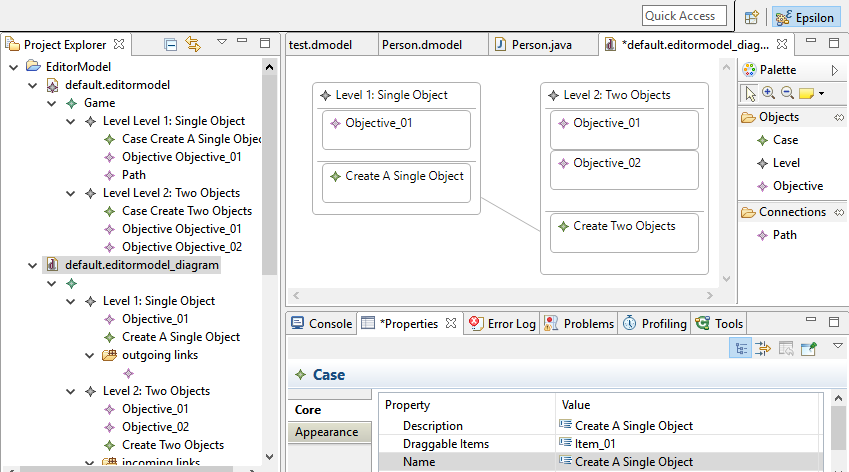
\includegraphics[width=\textwidth]{editor}}
\caption{Graphical editor for the gamification specification DSL \cite{Yohannis2016}.}
\label{editor}
\end{figure}

\begin{figure}[!t]
\centering
\frame{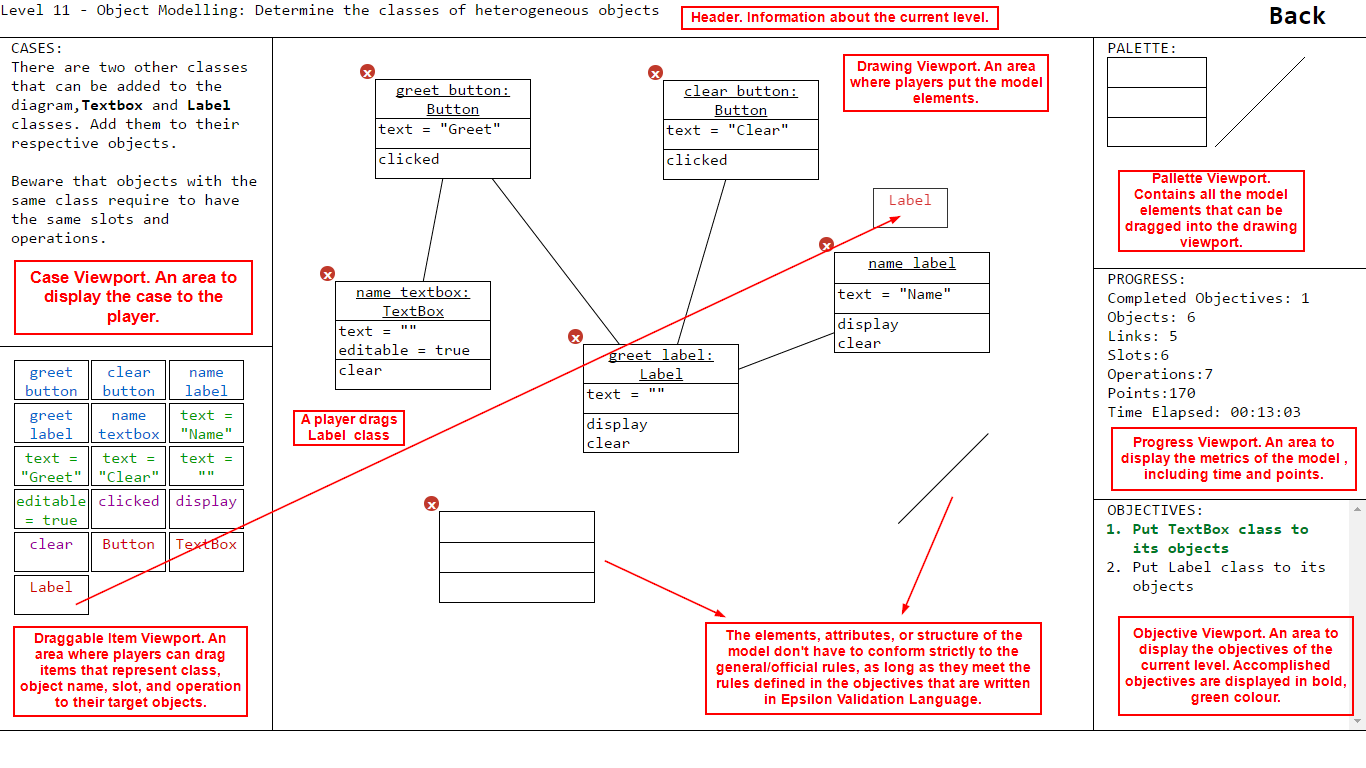
\includegraphics[width=\textwidth]{game-annotated}}
\caption{The display of the generated game \cite{Yohannis2016}.}
\label{game-annotated}
\end{figure}


Briefly describe and justify your  method(s) or research approach: You will also be expected to discuss these in the PR viva

Summarise the work that you have done so far, making clear how you are applying your method(s) or research approach.

Summarise any results you have obtained, and outline their significance: say how they contribute to your overall research questions or hypothesis.

Outline clearly how your research and its results will be evaluated.

\chapter{Research Plan}
\label{Research Plan}
We plan to complete literature study and develop prototype by the end of the first year (2016), and address gamification of modelling and metamodelling in the second year (2017) and third year (2018) respectively. 

\begin {table}[ht]
\caption {Research Timetable} 
\end{table}
\begin{figure}[ht]
\centering
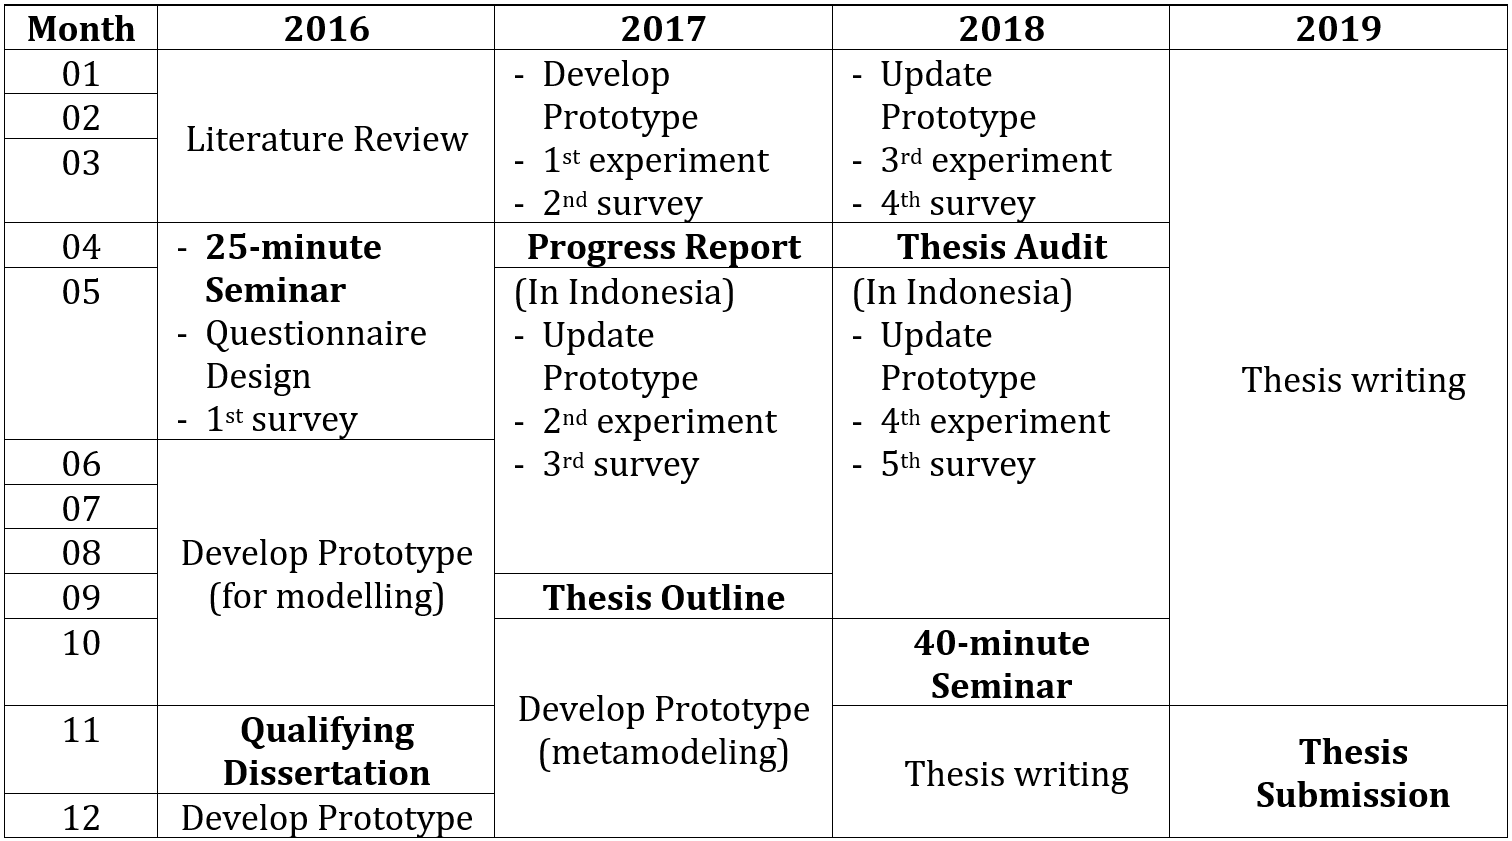
\includegraphics[width=\textwidth]{timetable}
\end{figure}

\chapter{References}
\label{References}

%\addcontentsline{toc}{chapter}{Bibliography}
\begingroup
\bibliographystyle{IEEEtran}
\renewcommand{\chapter}[2]{}%
\bibliography{references}
\endgroup

\chapter{Publications}
\label{Publications}
We have published papers in the following conferences or journals: 
\begin{enumerate}
 \item A. Yohannis, ``Gamification of software modelling learning,'' in
 \textit{the ACM/IEEE 19th International Conference on Model Driven Engineering Languages and Systems (MODELS 2016) Doctoral Symposium}. CEUR, 2016. \cite{Yohannis2016}.
\end{enumerate}




\begin{appendices}
\chapter{Preliminary Survey Data}
\label{chap:Preliminary Survey Data}

\begin{enumerate}
\item \textbf{If you think back to the time when you were just about to start the MODE module, what did you think you would find interesting in Model ­Driven Engineering?}
\begin{itemize}
\item Learning what MDE actually is. Had never heard of it so was intrigued.
\item I thought I would be provided with a high level approach to designing and managing software/critical systems.
\item Learning some tools to create auto­models.
\item Learning about ways of statically verifying that code conformed to a formal model, and using this to detect and automatically correct bugs learning about ways to automatically modify code based on changes made to a model.
\end{itemize}

\item \textbf{What did you find important in Model­ Driven Engineering?}
\begin{itemize}
\item Domain modelling ­ especially metamodels and the whole concept of abstract syntax. Regarding practicalities, the ability to use models to generate code is the most useful, along with creating DSLs.
\item Trying to learn the specific tools to pass the assessment. Not ideal as I wanted more generic
skill sets in this domain I could apply in my career, instead it was too focused on learning some niche features in Epsilon.
\item abstract thinking ­ validate the models ­ linking the model to real­life.
\item The ability to keep a formal model that the code has been verified to conform to throughout
an entire development process Automatic code generation modifcation based on a model.
\end{itemize}

\item \textbf{ Why did you decide to take the Model ­Driven Engineering module?}
\begin{itemize}
\item It was compulsory. I had no choice.
\item Compulsory.
\item well, I feel that everything around me has a certain model. Therefore, I felt learning about. Model­ Driven will increase my knowledge and experience in work. 
\item It seemed like it would be useful to learn a new approach to software engineering and skills that might be valuable in the industry in the future I was interested in generating and transforming code automatically and using a formal model for the structure of the code.
\end{itemize}


\item \textbf{ What would motivate you more to learn Model Driven Engineering?}
\begin{itemize}
\item Seeing the MDE approach being used to do something that would otherwise be much more tedious to do using more conventional means.
\item To see the benefit applied in the real world and how organisations have benefited from it. Then how can use these skills and adapt them to my needs?
\item If we link it to real­life examples, explore more other tools.
\item More use of it in industry More use with languages other than Java and different types of models such as ones that aren't based on UML/EMF.
\end{itemize}

\item \textbf{ Based on the answers that you’ve provided above (No. 1­4), what were the most basic, core underlying motives or needs that make you commit to learning Model­
Driven Engineering?}

\begin{itemize}
\item The ability to think at a higher level of abstraction and understand the concepts which link together a domain ­ especially, for example, programming languages. 
\item Passing the compulsory paper.
\item see some real­life examples and apply different models to see the differences. 
\item Learning skills which would be valuable in the SE industry in the future Learning something which would help with controlling the complexity of a sofware engineering process by making sure that code
conforms to a formally­defined model
\end{itemize}


\item \textbf{ What were the challenges that you found interesting in learning Model­Driven Engineering? Why?}
\begin{itemize}
\item One of the main challenges is in defining the abstract syntax for a DSL along with placing restrictions on its use through a validation language. There's a balance between trying to make the abstract syntax clean and easy to understand and modify vs. preserving the intended semantics.
\item None really, I found the assignment and practicals a tool based grind as opposed to a useful learning opportunity.
\item I sometimes felt that I could not apply all principles in the practicals­ especially on how we think abstract.
\item Working out how to best model a system, which had been defined informally, in EMF and EVL while keeping all its constraints intact and made it easily queryable and transformable was interesting.
\end{itemize}



\item \textbf{How did you manage to overcome these challenges?}
\begin{itemize}
\item By experimenting and going with what makes the most sense. If it is a structural issue with semantics, it is an abstract syntax issue. If it is something more peculiar, it is a validation issue.
\item By grinding through them.
\item I tried to train myself on other examples, but still, I could not link my models to real­life example( as a real project). 
\item The best way to learn this was from experience which was gained by completing all the practicals.
\end{itemize}


\item \textbf{ What were the challenges---the non­interesting challenges---that hindered or demotivated you in learning Model­Driven Engineering? Why?}
\begin{itemize}
\item Learning the Eclipse Modelling Framework, MOF, etc. wasn't fun. The most fun part was learning and use Emfatic with EGL/EGX and EOL in general. However, actually understanding the meta­metamodel and all the ecore stuff seemed pointless. You do not need to understand what EClass, EEnum, EString etc. are. It is just unnecessary detail that's very specific to
Eclipse and not something that you need to know even if you use Epsilon.
\item The focus on the tool as opposed to the high-level concepts and skill sets that would empower me to utilise model-driven engineering in the real world.
\item sometimes the tool itself, you need to re­track all your changes manually, no right answer or a good explanation why this model is good or bad.
\item Problems using eclipse, the shortcomings of EMF, lack of information available on the internet Eclipse is very large, complex and fragile. EMF/ UML ­style models, can be quite restrictive at times when modelling complex relationships, and often requires resorting to EVL. This is annoying because EVL constraints cannot be easily displayed on a diagram and two different languages/systems, EVL and EMF, are being used for similar things. Sometimes two very similar constraints exist where one can be modelled in EMF, and the other can not, and so requires EVL. Although there is a lot of very good documentation available about the languages in Epsilon, there is far less information on the internet about them than what is usually available for popular programming languages and it would be helpful if there was more.
\end{itemize}

\item \textbf{How did you overcome these challenges?}
\begin{itemize}
\item By ignoring them; once I realised they served no purpose for developers.
\item Reading up about the tools and grinding through them.
\item Asking questions, reading some examples in the Epsilon website forum.
\item Eclipse sometimes stops working but does this usually does not prevent the completion of tasks as most problems can be fixed by deleting the workspace directory and starting again, it simply wastes many time Things that could not be expressed in EMF were instead expressed using EVL. The required information about Epsilon could always be found by
asking classmates and asking lecturers, but this would not be possible if using these languages outside the university
\end{itemize}
\end{enumerate}

\chapter{Application of Deterding's Gameful Design Steps}
\label{Application of Deterding's Gameful Design Steps}


\section{Strategy}
\subsection{Define Target Outcome and Metrics}
\subsubsection{Outcome}
\begin{itemize}
\item Students that use the gamified learning perform better than traditional ones in software modelling.
\end{itemize}

\subsubsection{Metrics}
\begin{itemize}
\item Scores that they get from solving given software modelling problems.
\item Subjective opinions that learning through the gamified systems is better than the traditional ones. 
\item Model metrics of the models that they produce.
\end{itemize}

\subsection{Define Target Users, Context, Activities}
\subsubsection{Users}
Computer Science Undergraduate Students with some knowledge of object-orientation, ideally from both programming and design, and a good understanding of software engineering
\subsubsection{Context}
One term of software modelling course (Time) and in the context of university software modelling course (Place)
\subsubsection{Activities}
Modelling, metamodelling, and model management

\subsection{Identify Constraints and Requirements}
\subsubsection{Laws and regulations}
\begin{itemize}
\item Privacy regulation.
\end{itemize}
\subsubsection{Scope (time, budget, personnel)}
\begin{itemize}
\item Time. One term of software modelling.
\item People. Student of software modelling-related courses.
\item Budget. Available research budget.
\end{itemize}
\subsubsection{Technological requirements}
\begin{itemize}
\item Notebooks, computer desktops.
\item Internet connection.
\end{itemize}
\subsubsection{Others}
\begin{itemize}
\item Align with the existing learning models and software modelling teaching best practices.
\end{itemize}

\section{Research}
\subsection{Translate Users Activities into Behaviour Chains}
\subsubsection{Modelling}
\begin{itemize}
\item Real-world problems are given using textual description (or videos, interviews, images, etc.) 
\item Perform abstraction/identify relevant concepts (objects, values, attributes, and operations) according to the requirements 
\item Translate them into classes and relationships
\item Construct the model in the form of diagrams that represent the classes and relationships in different views (different diagrams)
\item Evaluate the models
\end{itemize}

\subsubsection{Meta-Modelling}
\begin{itemize}
\item Models are given using textual description (or videos, interviews, images, figures, etc.) 
\item Perform abstraction/identify relevant concepts (classes, relationships, attributes) of the models
\item Translate them into metamodel classes
\item Construct metamodel diagrams that represent the metamodel
\item Evaluate the metamodel
\end{itemize}

\subsubsection{Model Management}
\begin{itemize}
\item Problems are given using textual description (or videos, interviews, images, figures, etc.) 
\item Identify goals and constraints
\item Determine the model management operations:
Validation
\item Transformation (model-to-model, text-to-model, model-to-text)
Etc.
\item Refine the operations into more detail steps
\item Test
\item Execute
\end{itemize}

\subsection{Identify User Needs, Motivations, challenges}
\subsubsection{User needs}
\begin{itemize}
\item Master the software modelling.
\end{itemize}
\subsubsection{Motivations}
\begin{itemize}
\item Has competency in software modelling (Ability to solve problems and ability to produce artefacts or concrete products).
\item Fun, challenging.
\item Understanding the importance and advantages of software modelling.
\end{itemize}
\subsubsection{challenges}
\begin{itemize}
\item No fun, the presentation of software modelling is not interesting.
\item Abstraction is difficult, choosing the most relevant elements according to the requirements.
\item Heavy cognitive loads dealing with abstract concepts.
\end{itemize}

\subsection{Determine Gameful Design Fit}
\begin{itemize}
\item Does the activity connect to an actual user need? \textbf{Yes}
\item Is lacking motivation a central issue or opportunity (and not, e.g., poor usability)? \textbf{Both}
\item Does the target activity involve an inherent challenge with a learnable skill? \textbf{Yes}
\item Is affording experiences of competence the most effective and ef�cient way of improving motivation (and not, e.g., defusing fears)? \textbf{Yes}
\end{itemize}

\section{Synthesis}
\subsection{Formulate Activity, Challenge, Motivation  Triplets for Opportune Activities or Behaviours}

\subsubsection{What motivations energize and direct the activity?}
Software modelling mastery: solving problems and build abstract/concrete artefacts
\subsubsection{What challenges are inherent in the activity?}
\begin{itemize}
\item Abstraction: determine the most relevant objects and relationships between them
\item Diagramming: translate the resulting model into diagram
\item Algorithmic operation: much like programming but for model management
\end{itemize}
\subsubsection{What challenges can be removed through automation or improving usability?} 
\begin{itemize}
\item Simplify the real-world scenario to identify relevant objects
\item Simplify the diagramming processes
\item Simplify the algorithmic operations
\end{itemize}
\subsubsection{What challenges remain that the user can learn to get better at?}
Abstraction, diagramming, algorithmic operation
\subsubsection{What are the activities, challenges, and motives?}
\begin{itemize}
\item Activity: Construct model 
\item Challenge: abstraction, diagramming, algorithmic operation
\item Motive: fear to make mistakes (-), solving problems (+), create artefacts (+)
\end{itemize}

\section{Ideation}
\subsection{Brainstorming Ideas using Innovation Stems}
\subsubsection{Challenge lenses}
Onboarding, scaffolded challenge, varied challenge 
\subsubsection{Goal and motivation lenses}
Interim goals, viral calls to action, next base action, intrinsic rewards, secrets, templates, traces of others
\subsubsection{Action and object lenses}
Bite sized actions, interesting choices, limited choices, micro-flow, small pieces loosely joined, expressive objects, underdetermination, sensual objects
\subsubsection{Feedback lenses}
Immediate, juicy, actionable, appeal to motives, glanceable, varied, surprising, graspable progress.

\subsubsection{Example}
\begin{itemize}
\item Scaffolded challenge lens and Mastery motivation
How might we spark a sense of mastery in abstraction,  diagramming, and model operation?
\item How might we use scaffolded challenge to make the abstraction, diagramming, and model operation more enjoyable?
\item How might we spark a sense of mastery with scaffolded challenge?
\item How might we alleviate fear of making mistakes with scaffolded challenges?
\end{itemize}

\subsection{Prioritise Ideas}
Only one idea created so far. Learners are given a scaffolded series of problems to which they can exercise modelling, metamodelling, and model management. Motivating feedbacks to achieve mastery are integrated as well.

\section{Iterative Prototyping}
Prototyping is still on going work.


\chapter{Storyboard: Object Diagram}
\label{Storyboards}
\begin{itemize}
\item Objects
	\begin{itemize}
	\item Create single object (Level 01)
	\item Create two objects (Level 02)
	\item Create multiple objects (Level 03)
	\end{itemize}
\item Links (Relationships)
	\begin{itemize}
	\item Create single link (Level 04)
	\item Create multiple links (Level 05)
	\end{itemize}
\item Slots (Attributes)
	\begin{itemize}
	\item Determine a slot and its value (Level 06)
	\item Determine slots and their values (Level 07)
	\end{itemize}
\item Operations/Methods
	\begin{itemize}
	\item Determine operation (Level 08)
	\item Determine multiple (Level 09) operations
	\end{itemize}
\item Class of Objects
	\begin{itemize}
	\item Determine the class of homogeneous objects (Level 10)
	\item Determine different classes of heterogeneous objects (Level 11)
	\end{itemize}
\item Case Studies
	\begin{itemize}
	\item Reconstruct the model from the beginning (Level 12)
	\item Apply the skills on different/similar problem (Level 13)
	\end{itemize}
\end{itemize}

\begin{figure}[ht]
    \centering
    \subfloat[Level 01]{{ \frame{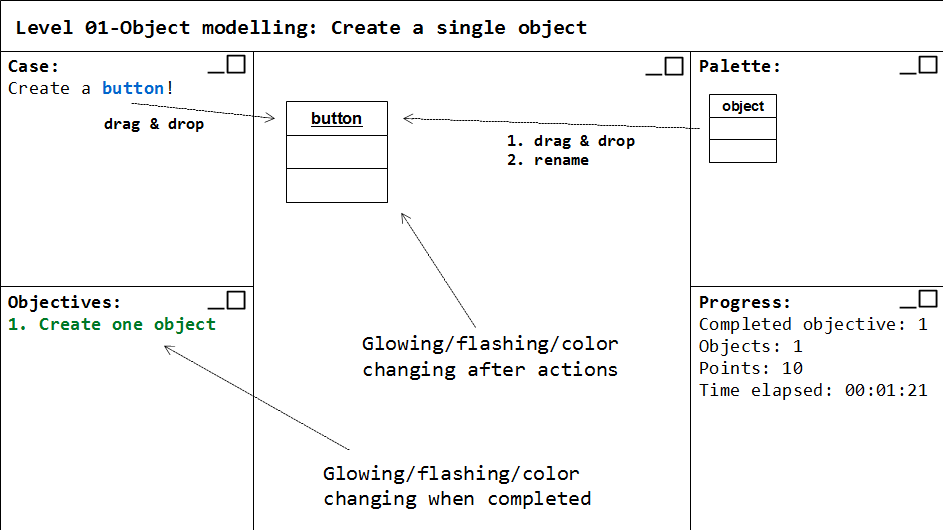
\includegraphics[width=7.16cm]{storyboard01}} }}
    \hspace{0cm}
    \subfloat[Level 02]{{ \frame{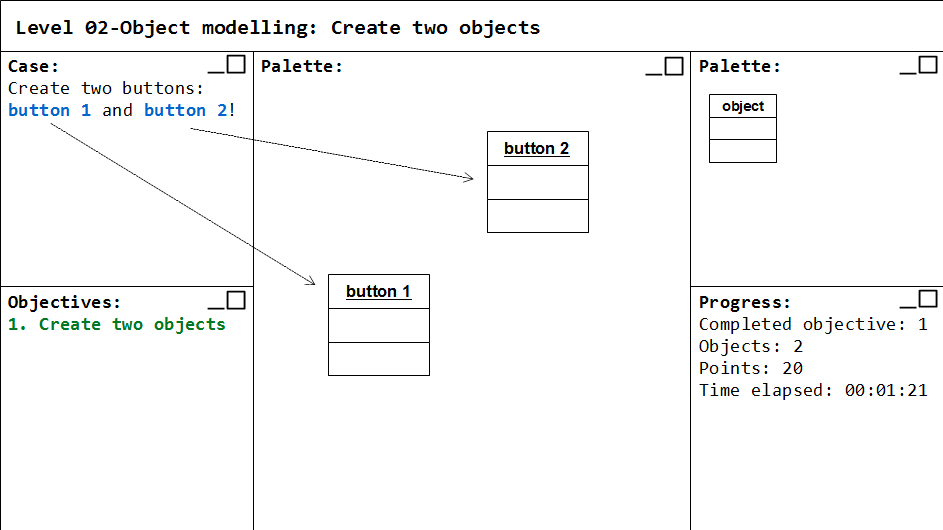
\includegraphics[width=7.16cm]{storyboard02}} }}
    \\
    \subfloat[Level 03]{{ \frame{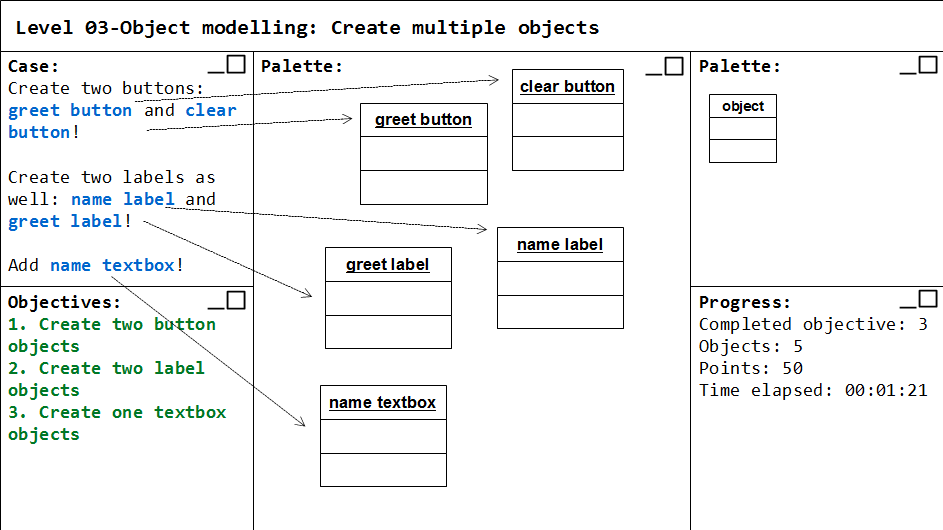
\includegraphics[width=7.16cm]{storyboard03}} }}
    \hspace{0cm}
    \subfloat[Level 04]{{ \frame{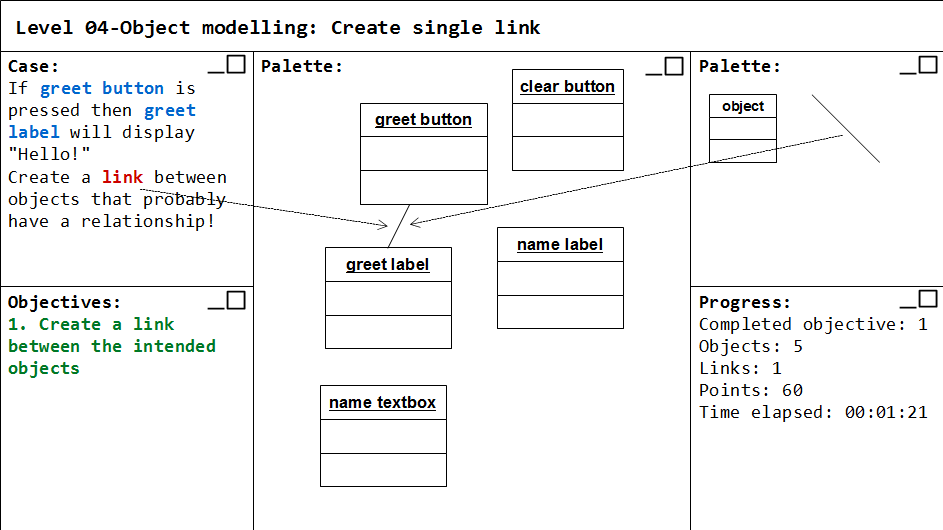
\includegraphics[width=7.16cm]{storyboard04}} }}
    \\
    \subfloat[Level 05]{{ \frame{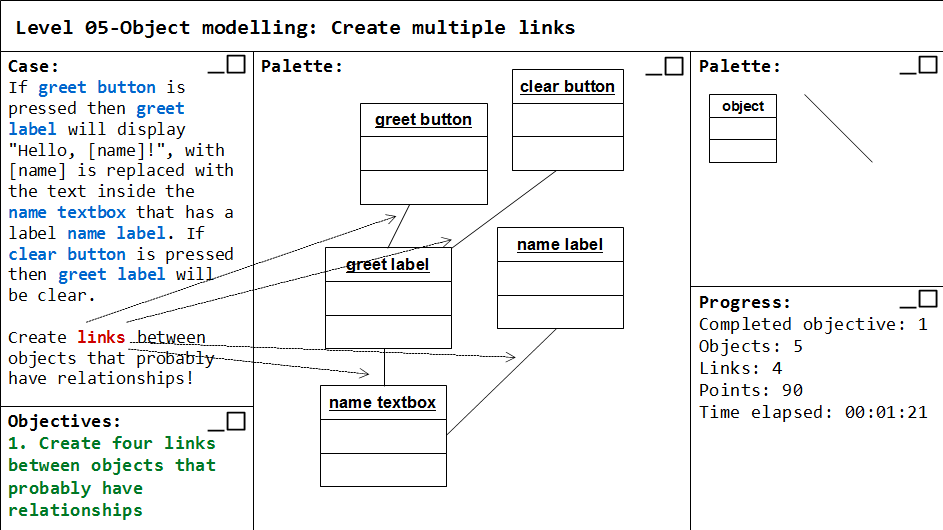
\includegraphics[width=7.16cm]{storyboard05}} }}
    \hspace{0cm}
    \subfloat[Level 06]{{ \frame{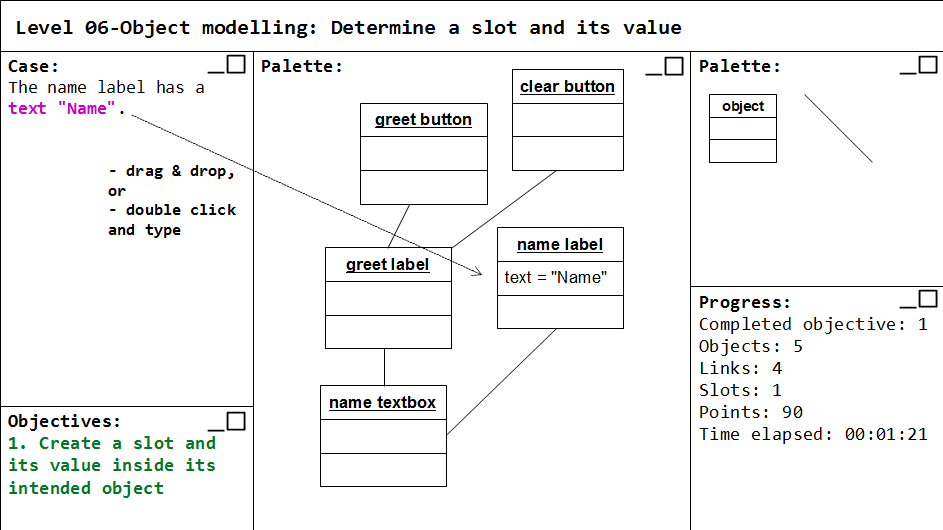
\includegraphics[width=7.16cm]{storyboard06}} }}
    
    
    
    \caption{Storyboard of Gamification of Object Diagram (part 1).}
    \label{storyboard-1}
\end{figure}


\begin{figure}[ht]
    \centering
    \subfloat[Level 07]{{ \frame{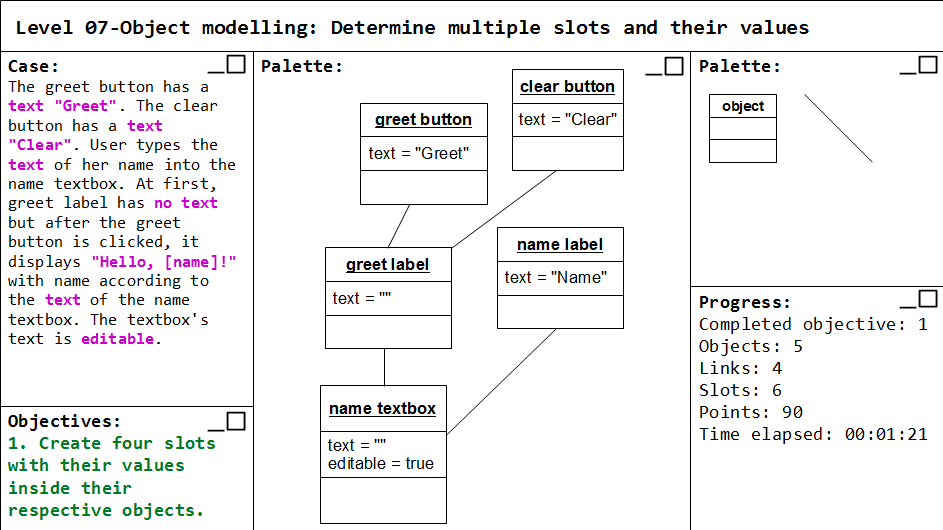
\includegraphics[width=7.16cm]{storyboard07}} }}
    \hspace{0cm}
    \subfloat[Level 08]{{ \frame{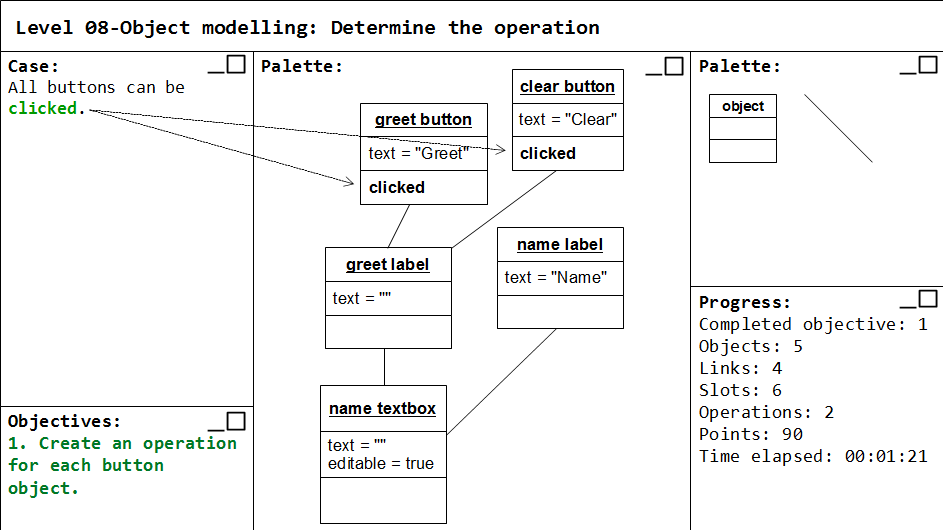
\includegraphics[width=7.16cm]{storyboard08}} }}
    \\
    \subfloat[Level 09]{{ \frame{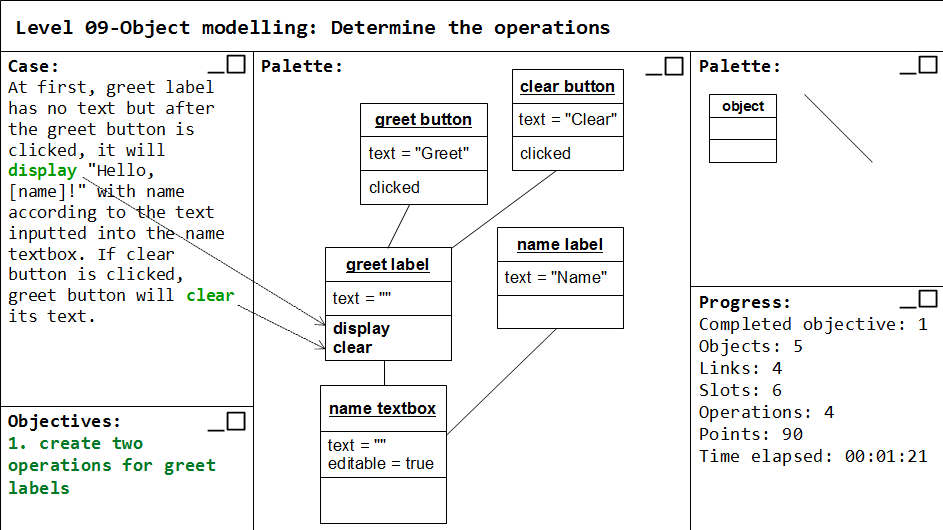
\includegraphics[width=7.16cm]{storyboard09}} }}
    \hspace{0cm}
    \subfloat[Level 10]{{ \frame{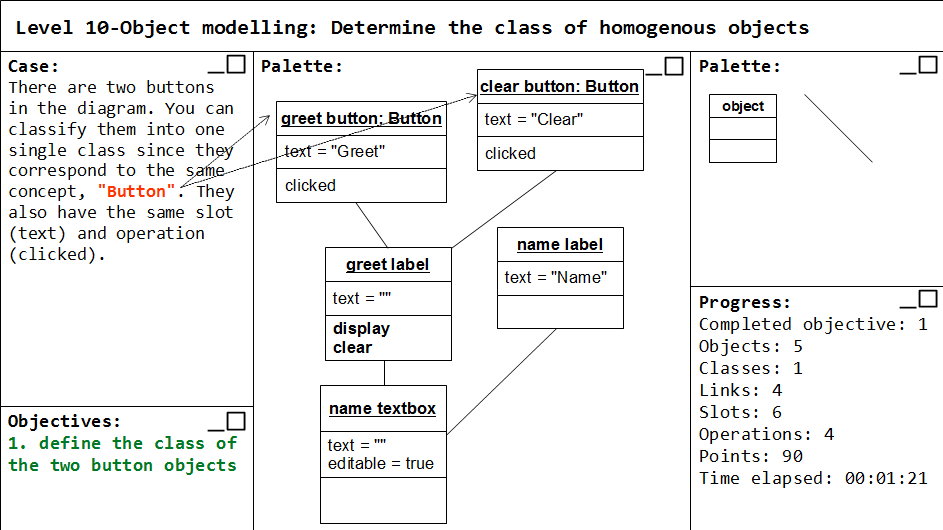
\includegraphics[width=7.16cm]{storyboard10}} }}
    \\
    \subfloat[Level 11]{{ \frame{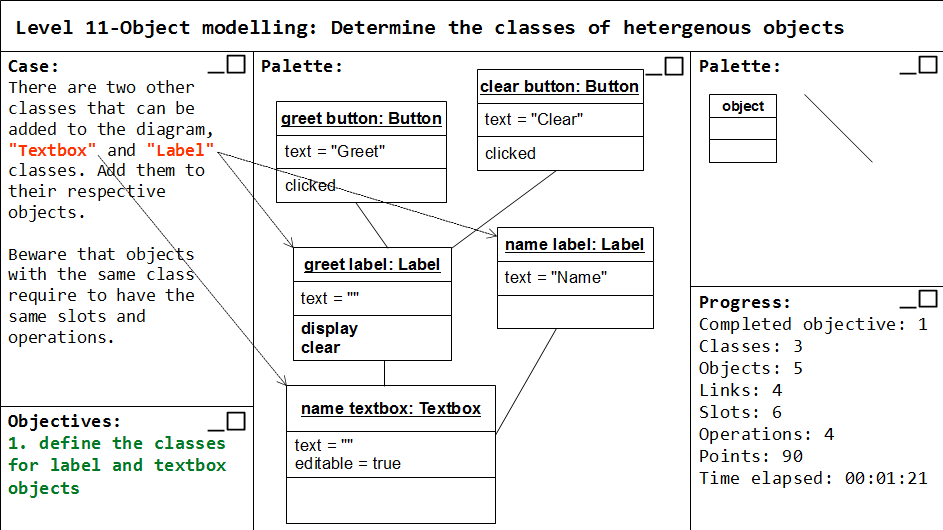
\includegraphics[width=7.16cm]{storyboard11}} }}
    \hspace{0cm}
    \subfloat[Level 12]{{ \frame{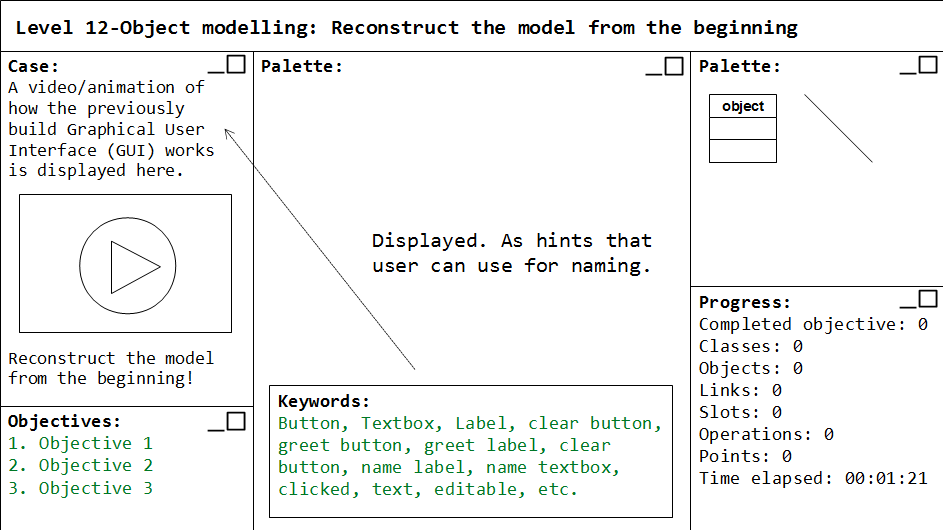
\includegraphics[width=7.16cm]{storyboard12}} }}
\caption{Storyboard of Gamification of Object Diagram (part 2).}
    \label{storyboard-2}
\end{figure}


\end{appendices}

\end{document}





